\documentclass{standalone}
\usepackage{tikz}
\usetikzlibrary{arrows.meta, positioning}

\begin{document}
	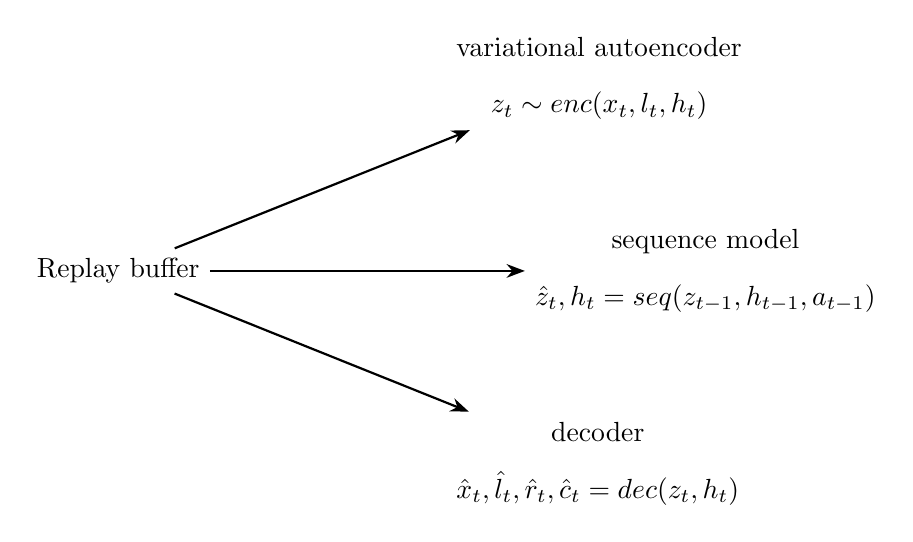
\begin{tikzpicture}[
		node distance=2cm,
		thick,
		>=Stealth,
		box/.style={rectangle, draw=none, align=center},
		equation/.style={align=center, font=\normalsize}
		]
		
		% Central node - Replay buffer
		\node[box] (replay) {Replay buffer};
		
		% Variational autoencoder branch (top right)
		\node[equation, above right=1.5cm and 3cm of replay] (vae) {
			variational autoencoder\\[0.3cm]
			$z_t \sim enc(x_t, l_t, h_t)$
		};
		
		% Sequence model branch (right)
		\node[equation, right=4cm of replay] (seq) {
			sequence model\\[0.3cm]
			$\hat{z}_t, h_t = seq(z_{t-1}, h_{t-1}, a_{t-1})$
		};
		
		% Decoder branch (bottom right)
		\node[equation, below right=1.5cm and 3cm of replay] (decoder) {
			decoder\\[0.3cm]
			$\hat{x}_t, \hat{l}_t, \hat{r}_t, \hat{c}_t = dec(z_t, h_t)$
		};
		
		% Arrows
		\draw[->] (replay) -- (vae);
		\draw[->] (replay) -- (seq);
		\draw[->] (replay) -- (decoder);
		
	\end{tikzpicture}
\end{document}